\documentclass[
	a4paper,
	12pt,
	twoside,
	%openright,
	DIV=12,
	BCOR=15mm,
	abstracton,
	parskip,
	listof=totoc,
	bibliography=totoc]{scrreprt}

% Headers and Footers
\pagestyle{headings}

% Font as serif
\setkomafont{disposition}{\normalcolor\bfseries}

\usepackage[utf8]{inputenc}
\usepackage[english]{babel}

\usepackage[lighttt]{lmodern}

\usepackage[numbers]{natbib}
\bibliographystyle{plainnat}
\usepackage[printonlyused]{acronym}

\usepackage{url}
\usepackage{hyperref}

\usepackage{graphicx}
\usepackage{rotating}
\usepackage{caption}
\usepackage{subcaption}

\usepackage{siunitx}

\usepackage{todonotes}
\usepackage[firstpage]{draftwatermark}
\SetWatermarkFontSize{12pt}
\SetWatermarkScale{8}
\SetWatermarkColor[gray]{0.95}

% Listings
\usepackage{scrhack}
\usepackage{listings}
\lstset{
	numbers=left,
	numbersep=4pt,
	xleftmargin=2em,
	xrightmargin=1em,
	framexleftmargin=1em,
	%aboveskip=2\parskip,
	%belowskip=\baselineskip,
	frame=tb,
	captionpos=b,
	breaklines=true,
	tabsize=3}
\lstset{
	basicstyle=\ttfamily\footnotesize,
	keywordstyle=\bfseries,
	%stringstyle=\color{gray},
	commentstyle=\color{gray}}
\renewcommand*{\lstlistlistingname}{List of Listings}

% Quotes before Chapter
\usepackage{epigraph}
\setlength{\epigraphwidth}{.6\textwidth}
\setlength{\epigraphrule}{0pt}

% Hurenkinder und Schusterjungen
\clubpenalty = 10000
\widowpenalty = 10000
\displaywidowpenalty = 10000

% Line Spacing Table
\renewcommand{\arraystretch}{1.6}

\begin{document}

\pagenumbering{roman}

\subject{
	Master Thesis \todo{openright}}
\title{
	Self-adaptation??? in Programmable Automation Controllers based on Hybrid
	Multi-Cores}
\author{
	Christoph Rüthing\\[-12pt]
	Student ID: 6619350}
\publishers{
	{\large Supervisors}\\[12pt]
	Prof. Dr. Marco Platzner\\
	Dipl.-Inf. Andreas Agne}
%\dedication{
%	Xilling Bing Bing}
\lowertitleback{
	Master Thesis\\
	\textbf{
		Self-adaptation in Programmable Automation Controller\\
		based on Hybrid Multi-Cores}\\[.5cm]
	University of Paderborn\\
	Faculty of Electrical Engineering, Computer Science and Mathematics\\
	Department of Computer Science\\
	Warburger Str. 100\\
	33098 Paderborn}

\maketitle

\cleardoublepage

%!TEX root = thesis.tex
\begin{abstract}
Modern industrial applications include a broad range of requirements, far
exceeding the traditional control and automation tasks. To accomodate these
new challenges, the so-called \ac{PAC} was introduced, combining the
advantages of traditional \acp{PLC} and \acp{PC}. The recent versions,
additionally, incorporate custom hardware for high-performance or low-latency
tasks, implemented on an \ac{FPGA}. The goal of this master project is to
develop an adaptive PAC, based on a heterogeneous reconfigurable
hardware/software architecture (ReconOS), with a focus on communication,
programmability and self-adaption strategies.
\end{abstract}

\chapter*{Declaration}

I hereby declare that I prepared this thesis entirely on my own and have not
used outside sources without declaration in the text. Any concepts or
quotations applicable to these sources are clearly attributed to them. This
thesis has not been submitted in the same or substantially similar version,
not even in part, to any other authority for grading and has not been
published elsewhere.\\[27pt]

\begin{center}
	\begin{tabular}{l p{0.1\textwidth} r}
		\cline{1-1}\cline{3-3}
		\begin{minipage}[t]{0.4\textwidth}
			\centering
			City, Date
		\end{minipage}
		&
		\begin{minipage}[t]{0.2\textwidth}
		\end{minipage}
		&
		\begin{minipage}[t]{0.4\textwidth}
  			\centering
  			Signatur
		\end{minipage}
	\end{tabular}
\end{center}

\tableofcontents
\listoffigures
\listoftables
\lstlistoflistings
%!TEX root = thesis.tex
\chapter*{List of Abbreviations}
\begin{acronym}
\acro{PAC}{Programmable Automation Controller}
\acro{PLC}{Programmable Logic Controller}
\acro{FPGA}{Field Programmable Gate Array}
\acro{CTOS}{commercial off-the-shelf}
\acro{CPU}{Central Processing Unit}
\acro{GPU}{Graphics Processing Unit}
\acro{DSP}{Digital Signal Processor}
\acro{PC}{Personal Computer}
\acro{ARC}{Automation Research Company}
\acro{COTS}{commercial off-the-shelf}
\acro{ASIC}{Application-Specific Integrated Circuit}
\acro{VHDL}{Very High Speed Integrated Circuit Hardware Description Language}
\acro{HDL}{Hardware Description Language}
\acro{SoC}{System on Chip}
\acrodefplural{SoC}[SoCs]{Systems on Chip}
\acro{HLS}{High Level Synthesis}
\acro{OS}{Operating System}
\acro{OSFSM}{Operating System Synchronization Finite State Machine}
\acro{OSIF}{Operating System Interface}
\acro{MEMIF}{Memory Interface}
\acro{POSIX}{Portable Operating System Interface}
\acro{TLB}{Translation Look-aside Buffer}
\acro{MMU}{Memory Management Unit}
\acro{RTL}{Register Transfer Level}
\acro{ISPS}{Instruction Set Processor Specification}
\acro{CMU-DA}{Carnegie-Mellon University Design Automation}
\acro{IP}{Intellectual Property}
\acro{RAM}{Random Access Memory}
\acro{FIFO}{First In First Out}
\acro{AXI}{Advanced eXtensible Interface Bus}
\acro{FSM}{Finite State Machine}
\acro{DSP}{Digital Signal Processor}
\acro{API}{Application Programming Interface}
\acro{RDK}{ReconOS Development Kit}
\acro{Tcl}{Tool Command Language}
\acro{LUT}{Lookup-Table}
\acro{MSB}{most significant bit}
\acro{LSB}{least significant bit}
\acro{6DoF}{six Degrees of Freedom}
\acro{CNC}{Computer Numerical Control}
\acro{CAD}{Computer Aided Design}
\acro{ITO}{Indium Tin Oxide}
\acro{ADC}{Analog-Digital-Converter}
\acro{SPI}{Serial Peripheral Interface}
\acro{Pmod}{Peripheral Module}
\acro{PID}{Proportional Integral Derivative}
\acro{PWM}{Pulse-Width Modulation}
\acro{IC}{Integrated Circuit}
\acro{I2C}[I\textsuperscript{2}C]{Inter-Integrated Circuit}
\acro{PID}{Proportional-Integral-Derivative}
\end{acronym}
\listoftodos

\cleardoublepage

\pagenumbering{arabic}

%!TEX root = thesis.tex
\chapter{Introduction}
%\epigraphhead[60]{\epigraph{``The future for PACs hinges on the incorporation
%of embedded technology''}{\textit{\citet{bel05}}}}

Modern industrial applications include a broad range of requirements, far
exceeding the traditional control and automation tasks. Buzzwords like
\emph{Industry 4.0} or the \emph{Internet of Things} emphasize the growing
demand of features. While a typical control system interfaces with simple
sensors and actuators, modern applications require more sophisticated features
like network connectivity, integration into enterprise systems or device
interoperability. To accommodate these new challenges and since the nowadays
dominating \ac{PLC} reaches its limits, the \ac{PAC} was introduced as the
next generation of control. It combines the reliability and robustness of a
\ac{PLC} with the advanced software capabilities of a \ac{PC}. By
incorporating state-of-the-art embedded technology like \acp{FPGA} and its
integration with general purpose processors on a single chip, these devices
eliminate the need for an expensive custom hardware and allow  the use of
\ac{CTOS} components, without loosing the benefits of executing time critical
control functions directly in silicon.

Unfortunately, the increasing complexity of such systems introduces new
challenges and demand convenient programming methods abstracting the
underlying low-level components, to make these devices accessible to a broad
range of developers. Classical ladder logic used for \acp{PLC} reaches its
limits and \ac{FPGA} technology is restricted to hardware designers capable of
handling low level programming languages like \ac{VHDL}. Because of its
acceptance in the field of software engineering and its eligibility to model
embedded systems composed of concurrently running tasks, the multithreaded
approach seems to be suitable as a convenient programming model for these
hybrid devices. The different threads specified by the developer are
distributed across the system's \ac{CPU} and \ac{FPGA} resources and
communicate via defined interaction mechanisms like message passing or shared
memory.\todo{Proposal Andreas}
\begin{itemize}
\item Develop a reconfigurable infrastructure for direct communication
between hardware threads. The new communication method should be integrated
into the ReconOS programming model as a new or as an extension of an existing
operating system abstraction. The choice of communication method should be
made by the runtime system in a way that is transparent for the programmer of
the hardeware thread.
\item Develop a toolchain that enables the use of \ac{HLS} for the creation of
ReconOS hardware threads. Investigate, how \ac{HLS} can be used to generate
the processing logic of a thread as well as the \ac{OSFSM}.
\item Implement a method to meassure the power consumption of the system.
Investigate means to meassure the on-chip power usage in a fine-grained way.
Investigate whether it is possible to meassure the power usage of individual
hardware threads.
\item Develop a \ac{PAC} that controlls a ball-on-plate application. The
application should contain components for the tracking of the ball, inverse
kinematics, and the required control algorithms. These components should be
implemented as a combination of hardware and software threads.
\item Use the previously developed application and components to meassure
thread performance, resource utilization and power consumption. Make the
application adapt to given goals and constraints by mechanisms like switching
on and off hardware and software threads, or switching between different
algorithms or implementations. Investigate different adaptation strategies
ranging from simple heuristics to more sophisticated methods involving machine
learning.
\end{itemize}
%!TEX root = thesis.tex
\chapter{Background and Related Work}
\label{chap:motivation}
This chapter gives an introduction into the relevant topics and motivates
the problems addressed in the rest of the thesis. It also includes
references to related work representing current research topics and points out
possible links. Beginning with an introduction into \acp{PAC} and their
history, the ReconOS framework is introduced, including a discussion on its
shortcomings and opportunities. Subsequently, modern \ac{HLS} approaches are
presented and the concept of self-adaptive systems is covered. Finally, the
contribution of this work is presented and motivated.

\section{\aclp{PAC}}
\aclp{PAC} are a relatively new class of controllers emerged in the past years
out of the discussions on advantages and disadvantages of \acp{PLC} compared
to \acp{PC} \citep{bel05}. The acronym \ac{PAC} itself was introduced by the
\ac{ARC} in 2001 \citep{pay13} to represent this next of generation
controllers. However, a strict definition to clearly identify a \ac{PAC} and
differentiate it from other \acp{PLC} is missing. The term is used as buzzword
for the automation vendor's marketing, but still reflects the increasing
demands by the modern industry and the evolution of automation controllers.

Since its origin in the 1960s \citep{par99}, the \ac{PLC} dominates the
control and automation market by providing high reliability, a well-known
programming model and industrial I/O. It is used for various automation tasks
in typically electromechanical processes, for example machinery or plant
control. Inspired by the hand-wired relay logic systems and wire-diagrams, the
ladder-logic programming eased the transition to the new technology. Figure
\ref{fig:plc} shows the basic structure of a \ac{PLC}, consisting out of input
and output ports and a program, implementing the control logic.
\begin{figure}[tb]
	\centering
	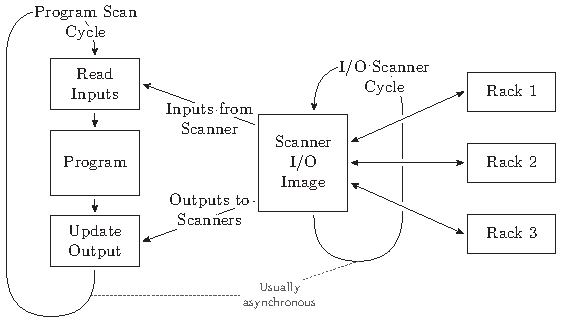
\includegraphics{../figures/plc}
	\caption{The \acs{PLC} program scan \citep[adapted from][]{par99}}
	\label{fig:plc}
\end{figure}
The input ports are typically connected to different sensors, for example
light barriers, level indicators or temperature sensors, while the output
ports control actuators like contactors or valves. Each time the program scan
is executed, the inputs are read and fed into the control logic, updating the
output ports accordingly. Note, that a \ac{PLC} does not control the system
continuously, but typically at a frequency of several $\SI{}{\kilo\hertz}$
\citep{par99}.

While the \ac{PLC} structure was designed for basic machine control, it
reaches its limits for more advanced applications requiring, for example,
extensive analog I/O, network connectivity, or enterprise integration. Back in
the 1980s and 1990s around 80\% of the industry's applications were solved by
traditional \acp{PLC} \citep{bel05}. This resulted in a growth of low-cost
systems and a discontinuity in controller technology. Engineers, targeting the
20\% of feature-rich applications, pushed the classical designs to its limits
and started evaluating different technology. They came up with \acp{PC} for
industrial control, offering advanced software capabilities, utilization of
\ac{COTS} components and graphical environments \citep{bel05}. However,
standard \acp{PC} are not ideal for industrial control applications, due to
missing robustness in rugged environments, stable operating systems and common
programming models. Finally, the engineers either omitted advanced
functionalities or deployed a coupled \ac{PC}/\ac{PLC} system. Without any
satisfactory solution, hardware vendors tried to fill up the gap by developing
a new class of controller, the so-called \acp{PAC}.

The \ac{PAC} combines the best features of \acp{PLC} and \acp{PC} in a single
device, by incorporating robustness and reliability with advanced software
capabilities as illustrated in figure \ref{fig:pac}.
\begin{figure}[tb]
	\centering
	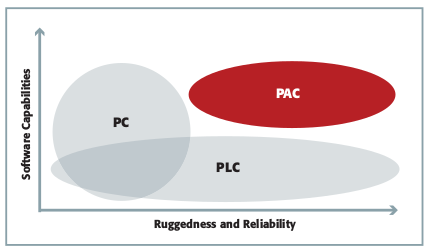
\includegraphics{../figures/pac}
	\caption{\acsp{PAC} compared to \acsp{PLC} and \acsp{PC} \citep[adapted from][]{bel05}}
	\label{fig:pac}
\end{figure}
However, vendors pursue different strategies to provide the advanced software
for complex applications. \citep{bel05}. Traditional \ac{PLC} companies
adjusted the existing scanning architecture and extended it by new
functionality. While the well-known architecture provides short development
cycles and eliminates the need of low-level knowledge by the engineers, it
still limits the flexibility and customizability of the system. On the other
hand, \ac{PC} vendors addressed the demand for advanced features by starting
with a general-purpose programming environment, which provides access to the
internals of the system and abstractions for commonly used operations. While
this approach allows extremely flexible solutions, it lacks the familiar
\ac{PLC} programming architecture, making application development more
demanding.

The flexible software architecture introduced for the \acp{PAC} enables
engineers to implement complex applications, without being restricted to a
fixed device structure. However, software implementations reach their limits
for high-performance or low-latency applications. These demands typically
result in custom hardware design, utilizing direct I/O connections and
parallel processing. While \acp{ASIC} are often not financially viable,
\acp{FPGA} are getting more and more ubiquitous \citep{VMB13}. \acp{FPGA}
consist out of configurable logic, interconnect and I/O blocks, which can be
programmed to implement arbitrary logic. While this technology seems to
perfectly fit into the concept of \acp{PAC}, especially with upcoming
integrated \acp{SoC}, it is limited to hardware designers capable of
programming in low-level languages like \ac{VHDL} and understanding the
architecture of the underlying system. Efficiently programming such a hybrid
system requires a high-level abstraction of hardware and software resources
\citep{ANA04} and a unified programming environment. Both topics are part of
ongoing research including programming models for hybrid multi-core systems
and high-level specifications of hardware logic.

\section{ReconOS for Hybrid Multi-Core Systems}
With increasing demand for high-performance embedded systems and upcoming
\acp{SoC}, integrating powerful general-purpose processors with reconfigurable
logic, convenient programming models are required to tap the full potential of
these hybrid systems \citep{ANA04,VMB13}. \ac{HLS} approaches allow the
synthesis from a high-level language and simplify the development of custom
hardware, but do not provide an abstraction for the underlying hardware
components at system level.

ReconOS addresses this problem and provides a unified execution environment
leveraging the well-established multithreaded programming model and extending
an existing \ac{OS} with hardware thread support \citep{AHK14}. The
multithreaded programming model is highly accepted in the software engineering
community and suitable for embedded applications \citep{ANA04} composed out of
concurrently running threads, synchronizing and exchanging data via
standardized \ac{OS} mechanisms, for example semaphores, mutexes or message
queues. The threads specified by the system developer are transparent against
their implementation and distributed across the \ac{CPU} and \ac{FPGA}
resources, while having symmetrical access to all communication mechanisms.
Figure \ref{fig:reconos_model} illustrates the concept of hardware and
software threads communicating via a standardized \ac{OS} interface.
\begin{figure}[tb]
	\centering
	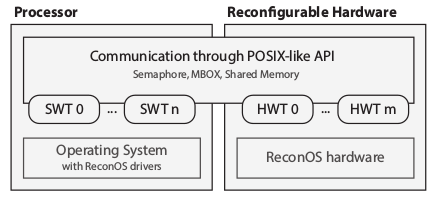
\includegraphics{../figures/reconos_model}
	\caption{The ReconOS programming model}
	\label{fig:reconos_model}
\end{figure}
The application structure remains at a high level and the partitioning can be
changed during development without additional effort. Furthermore, the
applications are portable between different platforms due to the defined
\ac{OS} interface.

To illustrate the concept of a ReconOS thread, consider the example sketched
in listing \ref{lst:swt}. It receives data via an incoming mailbox, processes
this data internally and writes back the result to an outgoing mailbox. Using
the predefined \ac{OS} functions for communication and synchronization, the
thread description separates internal processing from \ac{OS} interactions
\citep{AHK14}.
\begin{lstlisting}[
	language=C,
	caption={Exemplary ReconOS thread in C},
	label={lst:swt},
	morekeywords={THREAD_ENTRY,MBOX_GET,MBOX_PUT},
	float=tb
]
#include "reconos_thread.h"
#include "reconos_calls.h"

THREAD_ENTRY() {
	data_t data;

	while(1) {
		data = MBOX_GET(res_mbox_in);
		processing(&data);
		MBOX_PUT(res_mbox_out, data);
	}
}
\end{lstlisting}
This separation becomes even more apparent in the VHDL implementation shown in
listing \ref{lst:hwt}. The \ac{OSFSM} handles all requests to \ac{OS}
functions and controls the internal processing logic via handshaking signals.
For seamless integration, the ReconOS runtime provides a \ac{VHDL} library
wrapping all \ac{OS} functions as procedures with a guarding signal
\lstinline{done}, to condition the state transitions of the \ac{OSFSM}. This
signal allows blocking \ac{OS} calls to temporarily suspend the hardware
thread. While the \ac{OSFSM} mimics the sequence of \ac{OS} calls of the
software thread, the implementation of the internal processing may differ
significantly. It can benefit from all advantages of a custom \ac{FPGA} design
like fine-grained parallelism or specialized \ac{FPGA} resources.
\begin{lstlisting}[
	language=VHDL,
	caption={Exemplary ReconOS thread in VHDL},
	label={lst:hwt},
	morekeywords={MBOX_GET,MBOX_PUT},
	float=tb
]
OSFSM: process(HWT_Clk,HWT_Rst)
	variable done : boolean;
begin
	if rst = '1' then
		state <= GET_DATA;
		run <= '0';
		osif_reset(o_osif);
		memif_reset(o_memif);
	elsif rising_edge(clk) then
		case state is
			when GET_DATA =>
				MBOX_GET(i_osif, o_osif, res_mbox_in, data_in, done);
				if done then state <= PROCESSING; end if;
			when PROCESSING =>
				run <= '1';
				if rdy = '1' then
					run <= '0';
					if done then state <= PUT_DATA; end if;
				end if;
			when PUT_DATA =>
				MBOX_PUT(i_osif, o_osif, res_mbox_out, data_out, done);
				if done then state <= GET_DATA; end if;
		end case;
	end if;
end process OSFSM;
\end{lstlisting}

To support the transparent multithreading across the hardware/software
boundary, ReconOS implements a runtime architecture as shown in figure
\ref{fig:reconos_runtime}.
\begin{figure}[tb]
	\centering
	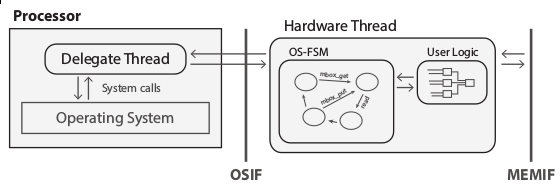
\includegraphics{../figures/reconos_hwt}
	\caption{The ReconOS runtime}
	\label{fig:reconos_runtime}
\end{figure}
It consists out of the application specific threads implemented either in
hardware or software, the \ac{OS} kernel executed on the main \ac{CPU} and the
ReconOS runtime components. While the host \ac{OS} provides scheduling, memory
management, low-level hardware access and the different programming model
objects published through the \ac{POSIX} API, the ReconOS runtime interfaces
with the \ac{OS} as software libraries and device drivers and implements
hardware components for communication and management.

The software threads are executed on the main \ac{CPU} as regular threads, for
example \ac{POSIX} threads -- and scheduled by the host \ac{OS}. To integrate
the hardware threads transparently into this system, ReconOS introduces the
concept of delegate threads. These lightweight software threads are connected
via the \ac{OSIF} to the hardware threads and provide an interface to the
\ac{OS}. Whenever a hardware thread needs to execute an \ac{OS} function, it
passes this request through the \ac{OSIF} to its associated delegate thread,
which executes the desired function and returns the result. From the \ac{OS}'
point of view, the hardware implementation is hidden behind the delegate
threads and the \ac{OS} only handles regular software threads. On the other
hand, the management of delegate threads is performed by the ReconOS runtime
and is completely hidden from the developer, seeing only the implemented
hardware and software threads. Although the delegate mechanism introduces an
overhead for executing \ac{OS} calls, it provides an exceptional transparency
regarding the threads implementation and execution mode and simplifies the
system design.

While the additional overhead for \ac{OS} calls is legitimated by the great
simplicity and portability of the design, access to shared memory is rather
performance critical. Handling memory requests via the delegate mechanism
would burden the processor with additional load and slow down the entire
system dramatically. To avoid this bottleneck, each hardware thread is
connected through a separate \ac{MEMIF} to the ReconOS memory subsystem. The
memory subsystem arbitrates the hardware thread's requests and performs the
memory access via the system bus. To support operating systems, like Linux,
providing virtual addressing, ReconOS implements a full-featured \ac{MMU}. It
translates virtual addresses by accessing the \ac{OS}' page tables and
accelerates translation by a \ac{TLB}. Similar to the \ac{OS} functions,
ReconOS provides \ac{VHDL} procedures to perform single-word or burst accesses
for convenient use.

Providing complete transparency against the implementation and execution mode
of threads, ReconOS simplifies the design process of hybrid multi-core
systems. However, hardware implementations are still limited to developers
familiar with \ac{FPGA} technology and low-level programming languages like
\ac{VHDL}. To lower these entry barriers and open the technology to a broader
range of developers, recent research explores \ac{HLS} to synthesize efficient
hardware out of high-level languages \citep{SWL13}. A common description for
both software and hardware implementations fits perfectly into the concept of
transparent multi-core systems \citep{CBN11}. A thread might be migrated at
runtime from software to hardware or vice versa, to fulfill requirements in,
for example, power consumption or performance. Such so-called self-adaptive
systems are also a hot topic in current research \citep{AHL14,HLP09}.

\section{\acl{HLS}}
%While the integration of hardware threads into the multithreaded programming
%model simplifies the design of hybrid multi-core systems at system level and
%presents a transparent model to the developer, the implementation of hardware
%threads is still challenging compared to that of software threads.
Developing custom hardware is not only limited to a subset of developers
capable of programming in low-level languages like \ac{VHDL}, but also time
consuming and error prone \citep{SWL13}. Traditional design methods and flows
make it difficult to debug and verify a system, resulting in increased costs
and reduced productivity. Recently, new \ac{HLS} tools are emerging, which try
to bridge the gap between hardware and software development. By synthesizing
hardware descriptions from high-level languages like C or C++, these tools
significantly lower the design time and make \ac{FPGA} designs accessible to a
broader range of developers \citep{PeTh05}. Relying on a correct synthesis,
\ac{HLS} induces fewer errors, less debugging and easier validation.

The idea of generating hardware from high-level languages is rather old, but
only state-of-the-art tools like Vivado HLS are sophisticated enough to
accelerate applications noticeably \citep{EcEc08,XSA10}. One of the first
pioneering \ac{HLS} system was developed in the 1970s \citep{DPS81} by the
Carnegie Mellon University, specifying a behavioural description in the
\ac{ISPS} language. Although \ac{CMU-DA} was rather experimental, it generated
considerable research interest in the following years. A variety of different
prototypes emerged and many algorithms targeting scheduling and allocation
problems were developed \citep{CBN11}. However, all these systems were not
widely adopted by the developers, since they build up on, at that time,
unreliable \ac{RTL} synthesis and uncommon languages. Since 2000, a new
generation of tools, focusing on C-based languages, emerged. Although the use
of C-based languages was doubted \citep{Edw06}, it enables hardware/software
co-design, co-simulation and the use of newest technology in software
compilers. To overcome the drawbacks of missing language constructs, modern
\ac{HLS} tools have introduced additional directives to make C inputs more
amenable to hardware synthesis \citep{CBN11}. Modern tools include commercial
programs like Vivado HLS from Xilinx or Catapult C from Calypto, as well as
academic prototypes like LegUp \citep{CCA11}. Due to its increasing
popularity, Xilinx Vivado HLS seems to be a promising system.

To synthesize an algorithm specified in a high-level language like C or C++,
\ac{HLS} extracts the control logic and operations, applies several
optimizations and generates an equivalent \ac{HDL} representation.
Additionally to the algorithmic synthesis, interfaces between different
entities and the outside world are generated. To control this transformation
process, the compilers support optimization directives to focus the \ac{HLS}
on particular objectives, for example performance, area or power consumption.%Typically, the algorithmic synthesis process includes scheduling, binding and
%control logic extraction. \citep{OCC14} At first, the control- and datapaths
%inferred by the code are extracted and transformed into an internal
%representation. Each program specifies a control path by its loops and
%conditional branches and a data path by its operations. Based on these
%information, \ac{HLS} performs scheduling and binding \citep{OCC14}.
%Scheduling determines, which operations are executed in a specific clock
%cycle and tries to find an optimal solution, based on clocking information,
%device technology specifications and user- defined directives. Binding then
%allocates hardware resources for each operation and decides on reuse of
%components. Finally, the control logic is extracted and an \ac{FSM} is
%generated, which sequences the scheduled operations.

During the synthesis, several optimizations are performed to increase the
performance of the generated \ac{RTL} representation. The most prominent
examples are loop unrolling and pipelining. Loop unrolling describes the
process of unfolding an iteration block into a sequence of statements,
allowing parallel execution \citep{SWL13}. Pipelining inserts registers into
combinational logic blocks to enable higher clock frequencies \citep{SWL13}.
The automated generation of pipelined structures simplifies the design-space
exploration and reduces development times dramatically. While hand-coded
piplines are error prone and hard to adapt, the \ac{HLS} developer has full
control over the generation via parameters specified in directives. Figure
\ref{fig:hls} show an example schedule generated by Vivado HLS out of a loop
adding 4 values. Each row indicates a single operation executed in one of the
states. Without any user defined directives, no unrolling takes place and a
regular loop is implemented as shown in figure \ref{fig:hls_n}, while the
\lstinline{#pragma HLS UNROLL} directive forces \ac{HLS} to unroll the loop as
shown in figure
\ref{fig:hls_u}.
%\begin{lstlisting}[
%	language=C,
%	caption={Exemplary HLS source},
%	label={lst:hls},
%	float=tb
%]
%#include "ap_cint.h"
%
%void top(uint32 d[4], uint32 *sum) {
%	uint32 acc = 0;
%
%	for (int i = 0; i < 4; i++)
%		acc += d[i];
%
%	*sum = acc;
%}
%\end{lstlisting}
\begin{figure}[tb]
	\centering
	\begin{subfigure}{0.49\textwidth}
		\centering
		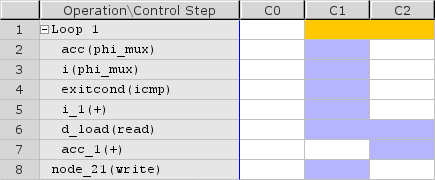
\includegraphics[width=0.97\textwidth]{../figures/hls_n}
		\caption{Inferred Schedule without Unrolling}
		\label{fig:hls_n}
	\end{subfigure}
	\begin{subfigure}{0.49\textwidth}
		\centering
		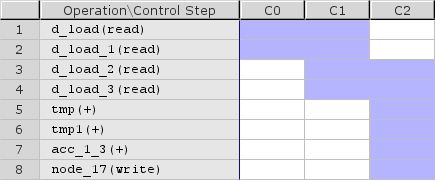
\includegraphics[width=0.97\textwidth]{../figures/hls_u}
		\caption{Inferred Schedule with Unrolling}
		\label{fig:hls_u}
	\end{subfigure}
	\caption{Scheduling in Vivado HLS}
	\label{fig:hls}
\end{figure}

\section{Self-adaptive Hybrid Multi-Core Systems}
Utilizing the potential of \ac{HLS} together with the multithreaded
abstraction layer allows to generate hardware and software threads from a
common specification \citep{CBN11}. This greatly simplifies system
implementation and design-space exploration and allows to find an optimal
configuration of threads. While a static configuration works perfectly for
predictable systems, it cannot be optimal in a dynamic environment with
rapidly changing demands, requiring an adaption at runtime.

Self-aware computing focuses on those kind of systems facing unprecedented
levels of system dynamics and requiring novel approaches to adaptivity. Recent
research investigates systems with so-called self-*properties \citep{SMC11},
which are capable of modifying their own behavior without external control in
reaction to or in anticipation of its dynamics. To be self-aware, a system
requires knowledge of phenomena internal and external to itself \citep{LCP11}.
Internal phenomena are captured by sensors like performance counters or
temperature sensors and external phenomena are recognized through the
environment. Both are handled by self-awareness engines, either private or
public, which are interacting with models of the system and environment.
Besides the self-awareness, requiring to gather data of the system and
environment, self-expression describes the ability to adapt to changes through
a self-expression engine and internal actuators. It is driven by objectives
and constraints given at design-time or dynamically at runtime.

With regard to hybrid multi-core systems, self-awareness and self-expression
allows the system to adjust its partitioning \citep{AHL14}. For example, a
thread might be migrated from software to hardware or additional threads might
be created, based on the dynamically changing processing demands
\citep{HLP09}. Utilizing dynamic reconfiguration features of modern \acp{FPGA}
permit even further adaption by completely reconfiguring the entire structure
and partitioning of the system.

\section{Contribution of this Work}
Due to the promising perspective for the use of reconfigurable devices in
\acp{PAC} and the ongoing research in hybrid multi-core systems, this thesis
evaluates the feasibility of such an approach.

To simplify the development of hardware threads and open the system to a
broader range of users, chapter \ref{chap:hls} discusses the integration of
Vivado HLS into the current toolchain to implement hardware threads. Since
Vivado HLS synthesizes from C code, the possibility of a common description
for hardware and software threads will be evaluated. Especially, the
generation of the \ac{OSFSM} will be investigated.

Following, the ReconOS framework will be extended to fit the needs for a
\ac{PAC} device. While the current delegate mechanism provides exceptional
transparency, it introduces a significant overhead for communication between
hardware threads. Especially for low-latency and high-performance
applications, this overhead lowers the overall performance and is not
acceptable. To utilize the full performance of a custom hardware
implementation, chapter \ref{chap:interconnect} presents a reconfigurable
interconnect, allowing direct communication between hardware threads through
existing or new \ac{OS} objects. The new communication method will be
integrated seamlessly into the ReconsOS programming model and provides
complete transparency to the developer, automatically selecting the
communication channel at runtime.

Utilizing the extended ReconOS framework, its feasibility for \acp{PAC} will
be evaluated in chapter \ref{chap:demonstrator} by implementing a 
Ball on Plate demonstrator, including ball tracking, inverse kinematics and
control algorithms. Additionally, the system will be able to self-adapt to
user constraints in power consumption or processing demand by reconfiguring
itself autonomously, for example switching between hardware and software
implementations or different algorithms. Building the demonstrator and
utilizing the new interconnect and \ac{HLS} features allows an extensive
evaluation and comparison to the current ReconOS framework.

\chapter{Interconnect}
\begin{itemize}
\item Motivation for interconnect (experiments, other projects, ...)
\item Always via software to slow
\item Consideration (resource limitations, ...)
\item Reconfigurable later on?
\end{itemize}
\section{Architectural Considerations}
\begin{itemize}
\item Comparison of different approaches
\item HThreads, ...?
\end{itemize}
\section{Implementation}
\section{Evaluation}
\begin{itemize}
\item measure time differences for old/new
\item show speedup/speeddown
\end{itemize}

\chapter{Integration of HLS}
\begin{itemize}
\item Motivation of HLS
\end{itemize}

\chapter{Demonstrator}

\cleardoublepage

\bibliography{thesis}

%!TEX root = thesis.tex
\chapter{Appendix}
\section{Evaluation of \acs{PID} Controller}
Although the scope of this thesis does not focuses on controller design and
tuning, a brief evaluation of the implemented \ac{PID} controller is given in
this section. By systematically exploring different values for the
\ac{PID} parameters, the final system applies $K_P = -0.09$, $K_I = 0$ and
$K_D = -28$. Figure \ref{fig:demo_pid} shows a tracking of the ball for two
applications.
\begin{figure}
	\centering
	\begin{subfigure}{0.49\textwidth}
		\centering
		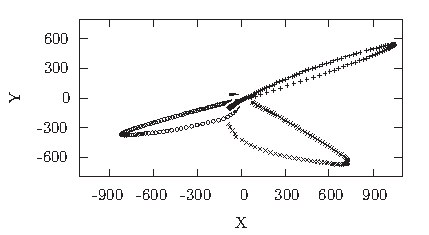
\includegraphics[width=\textwidth]{../figures/eval_pos}
		\caption{Balancing of ball in the center}
		\label{fig:eval_pos}
	\end{subfigure}
	\begin{subfigure}{0.49\textwidth}
		\centering
		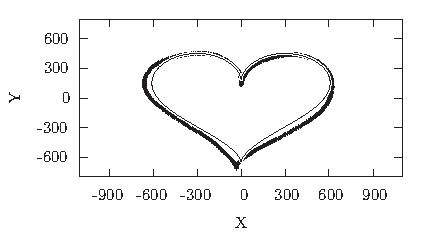
\includegraphics[width=\textwidth]{../figures/eval_traj}
		\caption{Following of a fixed trajectory}
		\label{fig:eval_traj}
	\end{subfigure}
	\caption{Captures of ball's movement controlled by \acs{PID} controller}
	\label{fig:demo_pid}
\end{figure}
For figure \ref{fig:eval_pos} the ball is balanced at the center of the plate
and any external disturbance is compensated, with the aim to keep the ball on
the plate. The figure shows a slight overshoot at the center and, due to a
missing integral term, never reaches the absolute center. Since the ball has a
relatively high initial friction, a large angle is needed to give the ball an
initial impulse. It then destabilizes and never reaches a resting position.
Therefore, a small inaccuracy for its final position is acceptable.
Additionally to the balancing of the ball in the center, figure
\ref{fig:eval_traj} shows an exemplary trajectory for the ball to follow.
Again, an inaccuracy from the desired trajectory in the direction of movement
is apparent. The trajectory is achieved by changing the target position of the
ball over time and adjusting the \ac{PID} controller to avoid the so-called
derivative kick.

\end{document}